\chapter{The accelerating universe}

\section{Introduction}

In 1929, Edwin Hubble discovered that the universe was expanding. At
the end of the 20 th century, astronomers made another stunning
discovery associated with the expansion of the universe. In 1998 two
independent projects obtained results showing that the expansion of
the universe was accelerating, a result that eventually led to Nobel
prizes for Perlmutter, Riess, and Schmidt in 2011. The two teams used
the same technique: measuring the distance and redshift of Type Ia
supernova. In this lab, you will work through some supernova data
looking for evidence of the accelerated expansion of the universe.

A supernova is essentially an exploding star. This ``explosion'' produces
a tremendous amount of light which then slowly fades over a period of
weeks to months. Measuring the light associated with the supernova
over time produces what is known as the supernova light curve. You can
use the following link to build some intuition about supernovae and
their light curves: \url{https://youtu.be/TY6Y5_7xQ8o}. An example of a
supernova light curve is shown in Figure~\ref{de:fig:light-curve}. The vertical axis is in ``magnitudes,'' the
standard astronomical measure of brightness where a larger magnitude
corresponds to a fainter object.

\begin{figure}
	\centering
	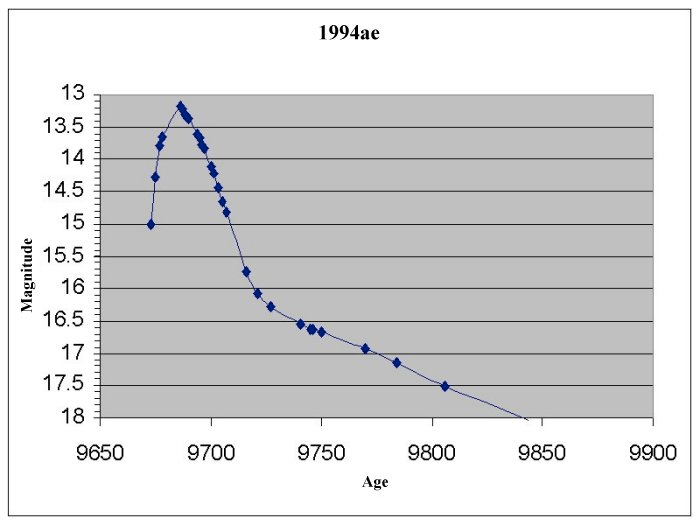
\includegraphics[width=0.7\textwidth]{dark-energy/light-curve-1994ae}
	\caption{Light curve for supernova 1994ae. The age is given in days.}\label{de:fig:light-curve}
\end{figure}

Supernova are used to measure distance in a manner similar to how we
measured distance in the Hubble lab. In the Hubble lab, we used the fact
that objects that are father away look smaller, that is, they subtend a
smaller angle on the sky. So, if we know the physical size of the object,
we can measure the object’s angular size and from that determine its
distance. For supernova, astronomers utilize the fact that objects that
are closer, look brighter, and objects that are farther away, look dimmer.
So, if we know the intrinsic brightness of an object (called its absolute
luminosity), we can then compare that to our measured brightness
(called its apparent brightness) to determine the object’s distance. This
concept for measuring distance is illustrated in Figure~\ref{de:fig:candles} showing how an object of a known brightness (or size) looks fainter
(smaller) when it is farther away.

\begin{figure}
	\centering
	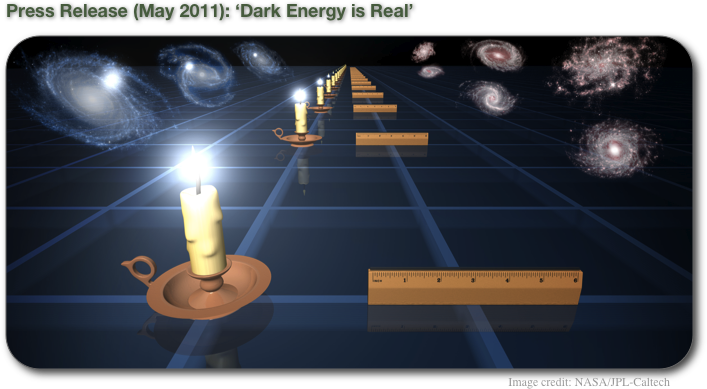
\includegraphics[width=0.8\textwidth]{dark-energy/candles}
	\caption{A method to determine the distance of an object. For objects with the same absolute luminosity, those are are further away will appear dimmer.}\label{de:fig:candles}
\end{figure}

The 1998 supernova teams studied Type Ia supernova because it is
possible to use the shape of the supernova light curve to deduce the
intrinsic brightness of the supernova. By comparing our inferred
intrinsic brightness with our measured apparent brightness, we can
then use the supernova to measure the distance.

\section{Making a supernova Hubble diagram}

The first activity for this lab is to make a Hubble diagram, like in the
Hubble lab, using Type Ia supernovae. Then you will analyze your Hubble diagram to qualitatively measure cosmic acceleration. Your data is in the Excel spreadsheet (available on Canvas in the Lab module in the compressed file DarkEnergyLab.zip) named SNe\_Reiss\_2004, and consists of distance moduli
and redshifts for 186 supernova from Reiss, et al., 2004.

As discussed above, the apparent magnitude of the supernova can be
used as a measurement of distance if we know the intrinsic brightness
(also called absolute brightness) of the supernova. In astronomy, we call
the difference between apparent and absolute brightness the “distance
modulus,” $\mu$, which is defined as
\begin{equation}
\mu = m - M \,,
\end{equation}
where $m$ is the apparent brightness (in
magnitudes), and $M$ is the absolute brightness (in magnitudes). The
distance to the object is related to the distance modulus by
\begin{equation}
 \textrm{distance} = 10^{(\mu-25)/5}\:\textrm{Mpc} \,.
\end{equation}

\begin{steps}
	\item In the spreadsheet, in a new column, calculate the distance for each supernova from the supernova’s
	distance modulus.
\end{steps}

After determining distances for objects, the next part of the Hubble
diagram involves making a measurement of the expansion of space. As
with the Hubble lab, we will estimate the expansion using the redshift
distortion of an object's spectrum. Recall that we measured the redshift
by looking for a specific spectral feature (either a dip or a peak) which
occurs at a known wavelength. A larger redshift indicates a faster recession velocity.

A constant expansion rate for the universe means that the amount of
expansion is proportional to the amount of time. Mathematically, we can
write this as
\begin{equation}
 \textrm{expansion } \propto \textrm{ time} \,.
\end{equation}
As expected, light emitted by more distant (and therefore older) objects
will undergo more expansion. This expansion leads to the redshifting
we discussed above. So, we can write that for a constant expansion rate,
the relationship between redshift and distance is
\begin{equation}\label{de:eq:hubble}
 \textrm{redshift} = \frac{H}{c} \times \textrm{distance} \,,
\end{equation}
where $c$ is the speed of light (300,000 km/s) and $H$ is called the Hubble
constant. This relation is known as “Hubble’s Law.” It describes a linear
relationship between redshift and distance, the two axes of the Hubble
diagram.

We can measure the expansion rate of the universe by using our Hubble
diagrams and fitting the data to Hubble’s law. The slope of the line that
fits the data will give a measurement of the Hubble constant, H, which
parameterizes the expansion rate of the universe.

\begin{steps}
	\item In the spreadsheet, sort data from closest to furthest. Then separately fit linear relationships to the 40 nearest and 40 furthest supernovae to obtain two Hubble constant measurements (Note that in Equation~\ref{de:eq:hubble}, the $y$-intercept is set to zero, so be sure to do this in your fit as well). Plot both linear relationships, as well as the data being fit, on a single graph. In order to see both sets of data more easily, set both axes to log scale to make a log-log plot.
	
	\item What value of the Hubble constant best fits the data for the 40
	closest supernova?
	
	\item What value of the Hubble constant best fits the data for the 40
	farthest supernova?
	
	\item How do these two results show that the expansion rate is accelerating?
	
	\item If the expansion rate is accelerating, what do you predict you
	should see if you fit data for 40 supernovae at intermediate
	distances?
	
	\item What value of the Hubble constant best fits the data for 40
	intermediate distance supernovae? Add this to your plot.
\end{steps}

\section{Finding and measuring supernovae}

Supernova are random events. In order to use supernova for
cosmological studies, astronomers must find them first. In this final
section of the lab, you will look at real data from the Dark Energy
Survey. You will search for a supernova and measure its light curve. Dr.
Daniel Scolnic, a former KICP fellow at the University of Chicago, has graciously
provided the images for this section.

\begin{steps}
	\item In the file you downloaded earlier, find the folder “SNe\_search” and
open the two image files SNe1\_search.jpeg and SNe2\_search.jpeg.
Compare these two images. These images correspond to pictures taken
of the same patch of sky on two different nights. A supernova is in one of
the images. Can you see it?
\end{steps}

In general, it is difficult to find supernova in a raw image of the sky
because of all the other objects in the image. Take a moment to look at
the different objects. Almost all of them correspond to stars
and galaxies.

Since the majority of objects in an image of the sky are not supernovae,
astronomers can try to remove them by generating a template image for
that patch of sky and then subtracting it from the image. Once these
non-supernova objects are removed (or mostly removed), it becomes
easier to search for supernovae.

\begin{steps}
	\item Open the file SNe1\_template.jpeg and compare it to SNe1\_search.jpeg.
\end{steps}
SNe1\_template.jpeg is the template file and it should look very similar
(though not exactly the same) to SNe1\_search.jpeg. Subtracting the two
yields a “difference” image which is file SNe1\_diff.jpeg.
\begin{steps}
	\item Open SNe1\_diff.jpeg.
\end{steps}
You should notice two things, 1) most of the features are now gone, and 2) the subtraction is imperfect. The imperfect subtraction introduces some artifacts in the differenced
image such as the spiderweb-like patterns and perfect geometric shapes
(like uniformly dark or bright squares and circles). You will note that
most of the artifacts from the imperfect subtraction are in locations
where there were very bright objects in the original image.

A supernova in the difference images will look like a round solid blob
that is very bright. Because a supernova is transient, the brightness of
the blob will not be the same in all images. In fact, there should be a few
images where there is no blob at all.

\begin{steps}
	\item Open the two difference images SNe1\_diff.jpeg and SNe2\_diff.jpeg.
	Compare these two difference images and identify the supernova.
	Remember, the supernova will look like a bright solid round blob in one
	of the images.
\end{steps}

Once you have found the supernova, the next step is to measure the
supernova light curve. We will do this using the DS9 software on your
computer.
\begin{steps}
	\item Open DS9 and press the “File” button to bring up the file
	menu. Press “open” and open the file 1-25-2014.diff.fits. This is the
	original file for the image with the supernova above.
\end{steps}

In DS9, you will need to press the “scale” button followed by the “zscale”
button so that the image will appear properly. You can drag the box to
look more closely at different parts of the image.
\begin{steps}
	\item Play around with the
	settings associated with the zoom, scale, and color buttons and examine
	different parts of the image.
	
	\item Find the supernova in this file (it is in the same location as in the earlier
	jpeg images). As you move the mouse around on top of the supernova,
	the “value” field will show you the value of the pixel underneath the
	mouse. Find the location on the supernova where this value is maximaland record the (X,Y) coordinates (the numbers for Image X and Y)
	below. We will use these (X, Y) coordinates as the coordinates for the
	supernova. Also record the pixel value.
	
	\item To measure the supernova’s light curve, load up each of the other *.fits
	files. Move the mouse to the (X, Y) coordinates you determined for the
	supernova and record the date and pixel value in your spreadsheet. Remember, the
	supernova is a transient object and it may not be present in all images.
	The filename tells you the date the image was taken.
	
	\item In the spreadsheet software, make a plot of the pixel value versus time. Make sure you use
	the date of the image to put your data in chronological order and to
	determine the time between each of the images.
\end{steps}

\section{Report checklist and grading}

Each item below is worth 10 points, and there is an additional 10 points for attendance and participation.

\begin{enumerate}
	\item Your Hubble diagram with all three sets of 40 supernovae and the three best-fit lines with their equations.
	
	\item Your three determinations of the Hubble constant (near, far, and mid), with work showing how you found them.
	
	\item Answers to questions 5 and 6.
	
	\item The table and plot of your experimental supernova light curve.
	
	\item Write
	one paragraph summarizing this lab. What is the significance and
	historical context of the discovery of cosmic acceleration (also called
	Dark Energy)? Why was it important? How does your analysis of the
	data in this lab demonstrate that the expansion rate of the universe is
	accelerating?
	
	\item A 100--200 word reflection on group dynamics and feedback on the lab manual. Address the following topics: who did what in the lab, how did you work together, what successes and challenges in group functioning did you have, and what would you keep and change about the lab write-up?
\end{enumerate}